% !TeX root = surprises.tex

\chapter{Langford's Problem}\label{c.langford}

%%%%%%%%%%%%%%%%%%%%%%%%%%%%%%%%%%%%%%%%%%%%%%%%%%%%%%%%%%%%%%%

\abstract*{Given the multiset of pairs of positive integers from $1$ to $n$, can they be arranged in a sequence such that for $1\leq i \leq n$ there are $i$ numbers between the two occurrences of $i$? This chapter presents two proofs of C. Dudley Langford's characterization of the values of $n$ for which a solution is possible. Worked-out solutions for $n=3,4$ are given.}

%%%%%%%%%%%%%%%%%%%%%%%%%%%%%%%%%%%%%%%%%%%%%%%%%%%%%%%%%%%%%%%

C. Dudley Langford\index{Langford, C. Dudley} noticed that his son had arranged colored blocks as shown in Fig.~\ref{f.langford}.
There is one block between the red blocks, two blocks between the blue blocks and three blocks between the green blocks. 
\begin{figure}[ht]
\begin{center}
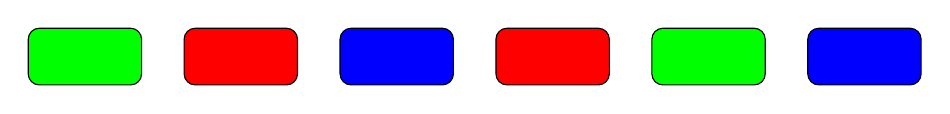
\begin{tikzpicture}[scale=.9]
\draw[rounded corners,fill=green] (0,0)  
  rectangle +(1.6cm,.8cm);
\draw[rounded corners,fill=red]   (2.2,0)
  rectangle +(1.6cm,.8cm);
\draw[rounded corners,fill=blue]  (4.4,0)
  rectangle +(1.6cm,.8cm);
\draw[rounded corners,fill=red]   (6.6,0)
  rectangle +(1.6cm,.8cm);
\draw[rounded corners,fill=green] (8.8,0)
  rectangle +(1.6cm,.8cm);
\draw[rounded corners,fill=blue]  (11,0)
  rectangle +(1.6cm,.8cm);
\end{tikzpicture}
\end{center}
\caption{Layout of blocks for Langford's problem}\label{f.langford}
\end{figure}

\begin{definition}[Langford's Problem $L(n)$] Given the multiset\footnote{A \emph{multiset} or \emph{bag} is like a set except that there may be more than one occurrence of an element.} of positive integers:
\[
\{1,1,2,2,3,3,\ldots,n,n\}\,,
\]
can they be arranged in a sequence such that for $1\leq i \leq n$ there are $i$ numbers between the two occurrences of $i$?
\end{definition}\index{Langford's problem}

Figure~\ref{f.langford} shows that 312132 is a solution for $L(3)$.

\smallskip

Section~\ref{s.langford-covering} restates Langford's problem using a mathematical formalism that facilitates solving the problem. Section~\ref{s.langford-theorem} characterizes values of $n$ for which $L(n)$ is solvable and presents two proofs of the theorem. The first proof which is relatively simple uses the technique of double-counting: counting the same value in two different ways and equating the resulting formulas. The second proof is a clever induction but the ``bookkeeping'' involved requires careful attention to the details. Section~\ref{s.langford-four} works out the solution for $L(4)$.

\section{Langford's Problem as a Covering Problem}\label{s.langford-covering}
\index{Langford's problem!covering@as a covering problem}
Langford's problem can be posed using an array. For $L(3)$ there are six columns, one for each position at which the six numbers can be placed. The rows are defined by the definition of the problem: the two occurrences of $k$ must have $k$ numbers between them. It is easy to see that there are four possible placements of $1$'s, three of $2$'s and two of $3$'s:

\begin{center}
\addtolength{\tabcolsep}{1mm}
\begin{tabular}{|c|c|c|c|c|c|c|}
\hline
Row&1&2&3&4&5&6\\\hline\hline
1&1&&1&&&\\\hline
2&&1&&1&&\\\hline
3&&&1&&1&\\\hline
4&&&&1&&1\\\hline
5&2&&&2&&\\\hline
6&&2&&&2&\\\hline
7&&&2&&&2\\\hline
8&3&&&&3&\\\hline
9&&3&&&&3\\\hline
\end{tabular}
\end{center}
To solve the problem, we need to select one row for the $1$'s in the sequence, one row for the $2$'s and one row for the $3$'s, such that if we stack these rows on top of each other, no column contains more than one number.

Row 9 needed not be considered because of symmetry: starting with row 9 just gives the reversal of the  sequence obtained by starting with row 8.

Row 8 is the only one containing $3$'s so it must be chosen and the sequence is 3\textvisiblespace \textvisiblespace \textvisiblespace 3\textvisiblespace. Any row with numbers in columns 1 and 5 can no longer be used, because only one number can be placed at each position. Let us denote the permissible and forbidden rows by:
\[\not\! 1,2,\not\! 3,4,\not\! 5, \not\! 6, 7, 8\,.\]

Row 7 is the only remaining row containing $2$'s so it must be chosen and the sequence is 3\textvisiblespace 2\textvisiblespace 3{}2. Deleting rows that can no longer be used gives:
\[\not\! 1,2,\not\! 3,\not\! 4,\not\! 5, \not\! 6, 7, 8\,.\]

Choosing the only remaining row, row 2, gives the solution 3{}1{}2{}1{}3{}2. Furthermore, the analysis has shown that this is the only solution, except for the symmetrical solution obtained by starting with row 9.
\begin{center}
\addtolength{\tabcolsep}{1mm}
\begin{tabular}{|c||c|c|c|c|c|c|}
\hline
Row&1&2&3&4&5&6\\\hline\hline
2&&1&&1&&\\\hline
7&&&2&&&2\\\hline
8&3&&&&3&\\\hline
\end{tabular}
\end{center}

\section{For Which Values of $N$ Is Langford's Problem Solvable?}\label{s.langford-theorem}

\begin{theorem} \label{thm.langford}
$L(n)$ has a solution if and only if $n=4k$ or $n=4k+3$.
\end{theorem}\index{Langford's problem!solvability, conditions for}

We prove the forward direction of the theorem. Proof~1 shows that if $L(n)$ has a solution then $n=4k$ or $n=4k+3$. Proof~2 shows the contrapositive: if $n=4k+1$ or $n=4k+2$ then $L(n)$ has no solution.

\begin{proof}[1] If the first occurrence of the number $k$ is at position $i_k$, the second occurrence is at position $i_k+k+1$. For example, in 3{}1{}2{}1{}3{}2, the solution for $L(3)$,  choosing $k=2$ gives $i_k=3$ and $i_k+k+1=3+2+1=6$.

The sum of the positions of all the numbers is:
\begin{eqnarray*}
S_n&=&\sum_{k=1}^{n}i_k+\sum_{k=1}^{n}(i_k+k+1)\\
& =& 2\sum_{k=1}^{n}i_k+\sum_{k=1}^{n}(k+1)\\
&=& 2\sum_{k=1}^{n}i_k+\frac{n(n+3)}{2}\,.
\end{eqnarray*}
But $S_n$, the sum of the positions, is simply $1+2+3+\cdots+2n$, so:
\[
S_n=\sum_{k=1}^{2n}k = \frac{2n(2n+1)}{2}\,.
\]
Equating the two formulas for $S_n$ gives:
\begin{eqnarray*}
2\sum_{k=1}^{n}i_k+\frac{n(n+3)}{2} &=& \frac{2n(2n+1)}{2}\\
\sum_{k=1}^{n}i_k &=& \frac{1}{2}\left(\frac{2n(2n+1)}{2} - \frac{n(n+3)}{2}\right) \\
&=& \frac{3n^2-n}{4}\,.
\end{eqnarray*}

The left-hand side is an integer since it is the sum of integers (the positions), so the right-hand side must also be an integer. When is $3n^3-n$ divisible by $4$? Factoring $3n^2-n$ gives $n(3n-1)$.

If $n$ is a multiple of $4$, the product is divisible by $4$.

When is $3n-1$ divisible by $4$? Any integer $n$ can be expressed as $n=4i+j$ for $j=0,1,2,3$. If $3n-1$ is divisible by $4$, then so is $3(4i+j)-1 = 12i+3j-1$. $12i$ is divisible by $4$. For $j=\{0,1,2,3\}$, $3j-1=\{-1,2,5,8\}$ is divisible by $4$ if and only if $j=3$, that is, $n=4i+3$.
\end{proof}

\newpage

To introduce the idea of the second proof consider what a solution for $n=4$ might look like. In the following tables the positions of the occurrences of 4 are 1 and 6, and the positions of the occurrences of 2 are 5 and 8. In both cases, one position is odd and the other is even. 
\[
\addtolength{\arraycolsep}{1mm}
\begin{array}{|c|c|c|c|c|c|c|c|}
\hline
1&2&3&4&5&6&7&8\\
\hline\hline
4&1&3&1&2&4&3&2\\\hline
*&&&&&*&&\\\hline
\end{array}
\hspace{3em}
\begin{array}{|c|c|c|c|c|c|c|c|}
\hline
1&2&3&4&5&6&7&8\\
\hline\hline
4&1&3&1&2&4&3&2\\\hline
&&&&*&&&*\\\hline
\end{array}
\]

Let $k=2m$ be an \emph{even} number. If $i$ is the position of the first occurrence of $k$, then the position of the second occurrence is $i+k+1$.
The sum of the positions is:
\[
i+(i+k+1)=2i+2m+1=2(i+m)+1\,,
\]
which is an odd number. For the sum of two numbers to be odd, one must be odd and the other even.

Let us now check the positions of the occurrences of odd numbers. The positions of the occurrences of 1 are 2 and 4, both even numbers, and the positions of the occurrences of 3 are 3 and 7, both odd numbers.
\[
\addtolength{\arraycolsep}{1mm}
\begin{array}{|c|c|c|c|c|c|c|c|}
\hline
1&2&3&4&5&6&7&8\\
\hline\hline
4&1&3&1&2&4&3&2\\\hline
&*&&*&&&&\\\hline
\end{array}
\hspace{3em}
\begin{array}{|c|c|c|c|c|c|c|c|}
\hline
1&2&3&4&5&6&7&8\\
\hline\hline
4&1&3&1&2&4&3&2\\\hline
&&*&&&&*&\\\hline
\end{array}
\]
Let $k=2m+1$ be an \emph{odd} number. The sum of the positions is:
\[
i+(i+k+1)=2i+2m+1+1=2(i+m+1)\,,
\]
which is an even number. For the sum of two numbers to be even, both must be odd or both even.

The positions $1,2,\ldots,2n-1,2n$ contain an equal number of even and odd positions. The two occurrences of a number in a row ``cover'' two positions. When the set of rows covers all the positions, they must cover an equal number of even positions and odd positions. Define the \emph{parity} of a set of rows to be the difference between the number of even and odd positions covered. Initially, the parity is zero, and if the problem has a solution, the set of rows in the solution also has zero parity.

When two occurrences of an even number are placed, they cover one even position and one odd position, so the parity remains the same:
\[
\addtolength{\arraycolsep}{1mm}
\begin{array}{|c|c|c|c|c|c|c|c|}
\hline
1&2&3&4&5&6&7&8\\
\hline\hline
4&1&3&1&2&4&3&2\\\hline
-1&&&&&+1&&\\\hline
\end{array}
\hspace{3em}
\begin{array}{|c|c|c|c|c|c|c|c|}
\hline
1&2&3&4&5&6&7&8\\
\hline\hline
4&1&3&1&2&4&3&2\\\hline
&&&&-1&&&+1\\\hline
\end{array}
\]
When two occurrences of an odd number are placed, the parity becomes $+2$ or $-2$, so we must be able to associate this pair with a pair of occurrences of \emph{another} odd number that are placed at positions that balance out the parity:
\[
\addtolength{\arraycolsep}{1mm}
\begin{array}{|c|c|c|c|c|c|c|c|}
\hline
1&2&3&4&5&6&7&8\\
\hline\hline
4&1&3&1&2&4&3&2\\\hline
&+1&&+1&&&&\\\hline
\end{array}
\hspace{3em}
\begin{array}{|c|c|c|c|c|c|c|c|}
\hline
1&2&3&4&5&6&7&8\\
\hline\hline
4&1&3&1&2&4&3&2\\\hline
&&-1&&&&-1&\\\hline
\end{array}
\]
We have shown that there can be a solution to Langford's problem if and only if \emph{there is an even number of odd numbers in $\{1,\ldots,n\}$}!
The theorem claims that if this is true then either $n=4k$ or $n=4k-1$, and if not then either $n=4k-2$ or $4k-3$.

\begin{proof}[2] 
The proof is by induction.
For the base case:
\begin{itemize}
\item $n=4k-3=1$. In $\{1\}$ there is an odd number of odd numbers and there is no solution.
\item $n=4k-2=2$. In $\{1,2\}$ there is an odd number of odd numbers and there is no solution.
\item $n=4k-1=3$. In $\{1,2,3\}$ there is an even number of odd numbers and we have seen that there is a solution.
\item $n=4k-0$. In $\{1,2,3,4\}$ there is an even number of odd numbers and Sect.~\ref{s.langford-four} gives a solution.
\end{itemize}

The inductive hypothesis is that the theorem is true for $\{1,\ldots,4k-j\}$, $k\ge 1$, $0\leq j\leq 3$ and we will prove that it is true for $n=4(k+1)-j$.

\begin{itemize}
\item Let us add $4k+1=4(k+1)-3$ to $\{1,\ldots,4k\}$. By the inductive hypothesis for $4k=4k-0$ there is an even number of odd numbers. $4(k+1)-3$ is odd so there is now an odd number of odd numbers and there is no solution.
\item Let us add $4k+2=4(k+1)-2$ to $\{1,\ldots,4k+1\}$. By the inductive hypothesis for $4k+1=4(k+1)-3$ there is an odd number of odd numbers. $4(k+1)-2$ is even so there is still an odd number of odd numbers and there is no solution.
\item Let us add $4k+3=4(k+1)-1$ to $\{1,\ldots,4k+2\}$. By the inductive hypothesis for $4k+2=4(k+1)-2$ there is an odd number of odd numbers. $4(k+1)-1$ is odd so there is an even number of odd numbers and a solution likely exists.
\item Let us add $4k+4=4(k+1)-0$ to $\{1,2,\ldots,4k+3\}$. By the inductive hypothesis for $4k+3=4(k+1)-1$ there is an even number of odd numbers. $4(k+1)-0$ is even so there is an even number of odd numbers and a solution likely exists.
\end{itemize}
\end{proof}

%%%%%%%%%%%% Solution for L(4) %%%%%%%%%%%%%%%%%%

\newpage

\section{Solution for $L(4)$}\label{s.langford-four}

\index{Langford's problem!solution of $L(4)$}
Here is the array for $L(4)$. Try to find the solution yourself.
\begin{center}
\addtolength{\tabcolsep}{1mm}
\begin{tabular}{|c||c|c|c|c|c|c|c|c|}
\hline
Row&1&2&3&4&5&6&7&8\\\hline\hline
1&1&&1&&&&&\\\hline
2&&1&&1&&&&\\\hline
3&&&1&&1&&&\\\hline
4&&&&1&&1&&\\\hline
5&&&&&1&&1&\\\hline
6&&&&&&1&&1\\\hline
7&2&&&2&&&&\\\hline
8&&2&&&2&&&\\\hline
9&&&2&&&2&&\\\hline
10&&&&2&&&2&\\\hline
11&&&&&2&&&2\\\hline
12&3&&&&3&&&\\\hline
13&&3&&&&3&&\\\hline
14&&&3&&&&3&\\\hline
15&&&&3&&&&3\\\hline
16&4&&&&&4&&\\\hline
17&&4&&&&&4&\\\hline
18&&&4&&&&&4\\\hline
\end{tabular}
\end{center}
By symmetry row 18 may be eliminated.

\smallskip

%$1,2,3,4,5,6,7,8,9,10,11,12,13,14,15,16,17$
\noindent Choose row 16 and the sequence is 4\textvisiblespace\textvisiblespace\textvisiblespace\textvisiblespace 4 \textvisiblespace\textvisiblespace.
Any row with an element in position $1$ or position $6$ can no longer be part of the solution.

$\not\! 1,2,3,\not\! 4,5,\not\! 6,\not\! 7,8,\not\! 9,10,11,\not\!\! 12,\not\!\! 13,14,15,16,\not\!\! 17$

\noindent Choose row 14 and the sequence is 4\textvisiblespace 3\textvisiblespace\textvisiblespace 4{}3\textvisiblespace.

$\not\! 1,2,\not\! 3,\not\! 4,\not\! 5,\not\! 6,\not\! 7,8,\not\! 9,\not\!\! 10,11,\not\!\! 12,\not\!\! 13,14, \not\!\! 15,16,\not\!\! 17$

\noindent Choose row 8. The sequence is 4{}2{}3\textvisiblespace 2{}4{}3\textvisiblespace.

$\not\! 1,\not\! 2,\not\! 3,\not\! 4,\not\! 5,\not\! 6,\not\! 7,8,\not\! 9,\not\!\! 10,\not\!\! 11,\not\!\! 12,\not\!\! 13,14, \not\!\! 15,16,\not\!\! 17$

\noindent All of the choices for 1's have been eliminated, so we must backtrack.

\smallskip

\noindent Instead of row 8 choose row 11 and the sequence is 4\textvisiblespace 3\textvisiblespace 2{}4{}3{}2.


$\not\! 1,2,\not\! 3,\not\! 4,\not\! 5,\not\! 6,\not\! 7,\not\! 8,\not\! 9,\not\!\! 10,11,\not\!\! 12,\not\!\! 13,14, \not\!\! 15,16,\not\!\! 17$

\noindent Choose row 2 and we have a solution 4{}1{}3{}1{}2{}4{}3{}2.

\smallskip

\noindent Let us continue backtracking to see if there is another solution.

\smallskip

\noindent Instead of row 14 choose row 15 and the sequence is 4\textvisiblespace \textvisiblespace 3\textvisiblespace 4\textvisiblespace 3.

$\not\! 1,\not\! 2,3,\not\! 4,5,\not\! 6,\not\! 7,8,\not\! 9,\not\!\! 10,\not\!\! 11,\not\!\! 12,\not\!\! 13,\not\!\! 14,15,16,\not\!\! 17$

\newpage

\noindent Row 8 must be chosen and the sequence is 4{}2\textvisiblespace 3{}2{}4\textvisiblespace 3.

$\not\! 1,\not\! 2,\not\! 3,\not\! 4,\not\! 5,\not\! 6,\not\! 7,8,\not\! 9,\not\!\! 10,\not\!\! 11,\not\!\! 12,\not\!\! 13,\not\!\! 14,15,16,\not\!\! 17$

\noindent All of the choices for 1's have been eliminated so again we backtrack.

\smallskip

\noindent Instead of row 16 choose row 17 and the sequence is \textvisiblespace 4\textvisiblespace \textvisiblespace \textvisiblespace\textvisiblespace 4\textvisiblespace.

$1,\not\! 2,3,4,\not\! 5,6,7,\not\! 8,9,\not\!\! 10,11,12,\not\!\! 13,\not\!\! 14,15,\not\!\! 16,17$

\noindent Choose row 15 and the sequence is \textvisiblespace 4\textvisiblespace 3\textvisiblespace\textvisiblespace 4{}3.

$1,\not\! 2,3,\not\! 4,\not\! 5,\not\! 6,\not\! 7,\not\! 8,9,\not\!\! 10,\not\!\! 11,\not\!\! 12,\not\!\! 13,\not\!\! 14,15,\not\!\! 16,17$

\noindent Row 9 must be chosen and the sequence is \textvisiblespace 4{}2{}3\textvisiblespace 2{}4{}3.

$1,\not\! 2,\not\! 3,\not\! 4,\not\! 5,\not\! 6,\not\! 7,\not\! 8,9,\not\!\! 10,\not\!\! 11,\not\!\! 12,\not\!\! 13,\not\!\! 14,15,\not\!\! 16,17$

\noindent All of the choices for 1's have been eliminated. We can backtrack one last time. 
%$1,\not\! 2,3,4,\not\! 5,6,7,\not\! 8,9,\not\! 10,11,12,\not\! 13,\not\! 14,15,\not\! 16,17$

\smallskip

\noindent Instead of row 15 choose row12 and the sequence is 3{}4\textvisiblespace \textvisiblespace 3\textvisiblespace 4.

$\not\! 1,\not\! 2,\not\! 3,\not\! 4,\not\! 5,\not\! 6,\not\! 7,\not\! 8,9,\not\!\! 10,\not\!\! 11,12,\not\!\! 13,\not\!\! 14,\not\!\! 15,\not\!\! 16,17$

\noindent Again, all of the choices for 1's have been eliminated.

\medskip

\noindent Therefore the only solution is $41312432$.

\subsection*{What Is the Surprise?}

The source of the inspiration for a mathematical theorem can be surprising. Langford noticed a pattern in his son's colored blocks which led to the interesting Thm.~\ref{thm.langford}. Students should also be introduced to the fact that a theorem  can have many completely different proofs.

\subsection*{Sources}
This chapter is based on \cite{miller}. \cite{davies} shows how to find a solution for $n=4k$ and $n=4k+3$.
